% !TeX program = lualatex
% !TeX root = luaking.tex
% !TeX encoding = UTF-8
% !TeX spellcheck = cs_CZ
%---------------------------------------------------------------------------------------------------
% file fey1ch20.tex
%---------------------------------------------------------------------------------------------------
%=========================== Kapitola: Rotace v prostoru ===========================================
\setchaptertoc
\chapter{Rotace v prostoru}\label{fyz:IchapXX}
  \section{Momenty sil v prostoru}\label{fyz:IchapXXsecI}
    V této kapitole se budeme zabývat jedním z nejpozoruhodnějších a nejzábavnějších důsledků
    mechaniky - chováním rotujícího tělesa. Za tím účelem musíme nejdříve rozšířit matematickou
    formulaci rotačního pohybu, pojmy moment hybnosti, moment síly atd. na trojrozměrný prostor.
    Tyto rovnice nebudeme používat v jejich úplné obecnosti, ani nebudeme studovat všechny jejich
    důsledky, neboť by nám to zabralo mnoho let a my se brzy musíme věnovat jiným tématům. V úvodním
    kurzu můžeme uvést jen základní zákony a aplikovat je na několik mimořádně zajímavých příkladů.

    Nejdříve si všimněme, že máme-li rotaci ve třech rozměrech, ať už jde o tuhé těleso nebo o
    nějaký jiný systém, pak to, co jsme odvodili v dvojrozměrném případě, stále platí. Stále tedy
    platí, že \(xF_y – yF_x\) je moment síly „v rovině \(xy\)“ nebo moment síly „kolem osy \(z\)“.
    Ukáže se i to, že tento moment síly je roven rychlosti změny \(xp_y - yp_x\), neboť kdybychom se
    vrátili k odvození rovnice (\ref{fyz:eq663}) z Newtonových zákonů, viděli bychom, že nemusíme
    předpokládat rovinný pohyb; když diferencujeme \(xp_y – yp_x\), dostaneme \(xF_y – yF_x\), takže
    tato věta stále platí. Veličinu \(xp_y – yp_x\) nazýváme momentem hybnosti příslušejícím rovině
    \(xy\) nebo momentem hybnosti vzhledem k ose \(z\). Protože toto platí, můžeme si vzít jakoukoli
    jinou dvojici souřadnicových os a odvodit další rovnici. Vezměme si rovinu \(yz\) a ze symetrie
    je jasné, že když prostě dosadíme \(y\) za \(x\) a \(z\) za \(y\), dostaneme pro moment síly s
    \(yF_z –  zF_y\) a \(yp_z-zp_y\) bude moment hybnosti spojený s rovinou \(yz\). Samozřejmě,
    mohli bychom vzít ještě jinou rovinu, rovinu \(zx\), a pro ni bychom dostali
    \begin{equation*}
      zF_x - xF_z = \der{ }{dt}(zp_x - xp_z).
    \end{equation*}

    je zcela jasné, že tyto tři rovnice lze odvodit pro pohyb jedné částice. Navíc, kdybychom výrazy
    jako \(xp_y - yp_x\) sečetli pro mnoho částic a součet nazvali celkovým momentem hybnosti, měli
    bychom tři výrazy pro tři roviny \(xy\), \(yz\) a \(zx\). Kdybychom totéž provedli i se silami,
    mohli bychom hovořit o momentu síly v rovině \(xy\), \(yz\) i \(zx\). Dostali bychom poznatek,
    že vnější moment síly příslušející kterékoli rovině je roven rychlosti změny momentu hybnosti
    příslušejícímu této rovině. Toto je zobecnění našich poznatků o dvojrozměrném případu.

    Někdo by ale mohl říci: „Ale existuje více rovin! Nemůžeme vzít nějakou jinou rovinu pod nějakým
    jiným úhlem a vypočítat moment síly v této rovině? Protože bychom pro každou takovou rovinu
    museli napsat další sérii rovnic, měli bychom velmi mnoho rovnic!“ Kupodivu se ukazuje, že
    stačí, když v nějaké jiné rovině změříme \(x'\), \(F_{y'}\) atd. a vypočteme kombinaci
    \(x'F_{y'}-y'F_{x'}\), pak lze výsledek napsat jako \emph{kombinace} tří výrazů v rovinách
    \(xy\), \(yz\) a \(zx\). To není nic nového. Jìnými slovy známe-li tři momenty sil v rovinách
    \(xy\), \(yz\), \(zx\), potom lze moment sílyv libovolné rovině a příslušný moment hybnosti
    napsat jakojejich kombinace: 6 procent zjednoho, 92 procent z druhého atd. Tuto vlastnost si
    nyní rozebereme.

    Předpokládejme, že Petr určil všechny momenty síly a všechny momenty hybnosti v příslušných
    rovinách v souřadnìcích \(xyz\), ale Pavel má souřadnicové osy \(x'\), \(y'\), \(z'\), jež mají
    jiný směr. Abychom si to trochu zjednodušili, budeme předpokládat, že se pootočily jen osy \(x\)
    a \(y\). Pavlovy \(x'\) a \(y'\) jsou nové, ale \(z'\) je stejné jako \(z\). Má tedy nové roviny
    \(yz\) a \(zx\). Proto jeho momenty síly a momenty hybnosti jsou jiné. Například jeho moment
    síly v rovině \(x'y'\) bude \(x'F_{y'}-y'F_{x'}\), atd. Nyní musíme najít vztah mezi novými a
    starými momenty síly, tj. najít spojení mezi oběma souřadnicovými soustavami. Někdo možná
    poznamená: „To vypadá podobně, jako to, co jsme dělali s vektory.“ Ano, přesně to chceme
    provést. Ale pak může říci: „A není moment síly vlastně vektor?“ \emph{Ukáže se}, že je to
    vektor, ale to nemůžeme vědět dříve, než provedeme jeho analýzu. Každý krok nebudeme provádět
    podrobně, chceme jen naznačit, jak se do dělá. Momenty sil, které vypočítá Petr, jsou
    \begin{subequations}\label{fyz:eq710}
      \begin{align}
        N_{xy} &=  xF_y - yF_x, \label{fyz:eq710a}  \\
        N_{yz} &=  yF_z - zF_y, \label{fyz:eq710b}  \\
        N_{zx} &=  zF_x - xF_z. \label{fyz:eq710c}        
      \end{align}
    \end{subequations}

    Poznamenejme, že nedáme-li dostatečný pozor na souřadnice, můžeme v takovýchto výrazech dostat
    nesprávné znaménko. Proč nepíšeme \(N_{yz} = zF_y - yF_z\)? Souvisí to se skutečností, že
    souřadnicová soustava může být buď pravotočivá, nebo levotočivá. Zvolíme-li si (libovolně)
    znaménko pro \(N_{xy}\), můžeme správné vyjádření dalších dvou veličin vždy najít záměnou
    \(xyz\) v jednom z pořadí
    \begin{equation*}
      x \rightarrow y \rightarrow z \rightarrow x
    \end{equation*}
    nebo
    \begin{equation*}
      x \rightarrow z \rightarrow y \rightarrow x.
    \end{equation*}
    Pavel ve své soustavě vypočítá takovéto momenty sil
    \begin{subequations}\label{fyz:eq711}
      \begin{align}
        N_{x'y'} &=  x'F_{y'} - y'F_{x'}, \label{fyz:eq711a}  \\
        N_{y'z'} &=  y'F_{z'} - z'F_{y'}, \label{fyz:eq711b}  \\
        N_{z'x'} &=  z'F_{x'} - x'F_{z'}. \label{fyz:eq711c}        
      \end{align}
    \end{subequations} 
    Předpokládáme, že jedna souřadnicová soustava je vzhledem k druhé pootočena o pevný úhel
    \(\Theta\), přičemž osy \(z\) a \(z'\) jsou totožné. (Tento úhel \(\Theta\) nemá nic společného
    s rotací předmětů nebo s tím, co se děje v dané souřadnicové soustavě. Určuje jen vztah mezi
    souřadnicovými osamì jednoho a souřadnicovými osamì druhého pozorovatele, přičemž předpokládáme,
    že je konstantní.) Souřadnice v těchto dvou systémech souvisí navzájem takto:
    \begin{subequations}\label{fyz:eq712}
      \begin{align}
        x' &=  x\cos\Theta + y\sin\Theta, \label{fyz:eq712a}  \\
        y' &=  y\cos\Theta - x\sin\Theta, \label{fyz:eq712b}  \\
        z' &=  z.                         \label{fyz:eq712c}        
      \end{align}
    \end{subequations} 
    Podobně, protože síla je vektor, transformuje se do nového systému stejně jako \(x\), \(y\),
    \(z\), protože veličina je vektorem tehdy a jen tehdy, kdy její různé složky se transformují
    jako \(x\), \(y\), \(z\)
    \begin{subequations}\label{fyz:eq713}
      \begin{align}
        F_{x'} &=  F_x\cos\Theta + F_y\sin\Theta, \label{fyz:eq713a}  \\
        F_{y'} &=  F_y\cos\Theta - F_x\sin\Theta, \label{fyz:eq713b}  \\
        F_{z'} &=  F_z.                           \label{fyz:eq713c}        
      \end{align}
    \end{subequations} 
    Dosazením do (\ref{fyz:eq711}) za \(x'\), \(y'\), \(z'\) z (\ref{fyz:eq712}) a za \(F_{x'}\),
    \(F_{y'}\), \(F_{z'}\), z (\ref{fyz:eq713}) můžeme nyní snadno zjistit, jak se transformují
    momenty síly. Tak dostáváme dlouhý výraz pro \(N_{x'y'}\), v němž se ukáže na první pohled
    překvapující skutečnost, že se zredukuje na \(xF_y - yF_x\), v čemž poznáváme moment síly v
    rovině \(xy\)
    \begin{align}
      N_{x′y′}  &=(x\cosθ+y\sinθ)(F_y\cosθ−F_x\sinθ)− (y\cosθ−x\sinθ)(F_x\cosθ+F_y\sinθ) \nonumber\\
                &=xF_y(\cos2θ+\sin2θ)−yF_x(\sin2θ+\cos2θ)+ xF_x(−\sinθ\cosθ+\sinθ\cosθ)+ 
                  yF_y(\sinθ\cosθ−\sinθ\cosθ)                                            \nonumber\\
                &=xF_y−yF_x=N_{xy}.                                                \label{fyz:eq714}
    \end{align}
    Tento výsledek je jasný, neboť pootočíme-li naše souřadnice jen v rovině, pak otáčení kolem osy
    \(z\) se nezmění, neboť ani rovina se nezměnila! Zajímavější bude sledování výrazu \(N_{y′z′}\)
    neboť tu jde o novou rovinu. To, co jsme dělali s rovinou \(x'y'\), proveďme nyní s rovinou
    \(y'z'\). Dostáváme
    \begin{align}
      N_{y′z′}  &=(y\cosθ−x\sinθ)F_z− z(F_y\cosθ−F_x\sinθ)  \nonumber  \\
                &=(yF_z−zF_y)\cosθ+(zF_x−xF_z)\sinθ         \nonumber  \\
                &=N_{yz}\cosθ+N_{zx}\sinθ.                  \label{fyz:eq715}
    \end{align}
    Nakonec si zopakujme totéž pro rovinu \(z'x'\)
    \begin{align}
      N_{z′x′}  &=z(F_x\cosθ+F_y\sinθ)−(x\cosθ+y\sinθ)F_z   \nonumber  \\
                &=(zF_x−xF_z)\cosθ−(yF_z−zF_y)\sinθ         \nonumber  \\
                &=N_{zx}\cosθ−N_{yz}\sinθ.                  \label{fyz:eq716}
    \end{align}
    Chtěli jsme odvodit pravidlo,jak najít momenty síly v nových souřadnicích a už ho máme. Jak si
    lze toto pravidlo zapamatovat? Když si pozorně prohlédneme vztahy (\ref{fyz:eq714}),
    (\ref{fyz:eq715}) a (\ref{fyz:eq716}), vidíme, že mezi nimi a vztahy pro \(x\), \(y\) a \(z\)
    existuje úzká souvislost. Kdybychom \(N_{xy}\) označili jako \(z\)-ovou složku \(N\), pak
    (\ref{fyz:eq715}) bychom mohli chápat jako vektorovou transformaci, neboť \(z\)-ová složka se
    nezmění a tak to má být. Dáme-li podobně do souvislosti rovinu \(yz\) a \(x\)-ovou složku našeho
    nového vektoru a rovinu \(zx\) s \(y\)-ovou složkou tohoto vektoru, pak tyto výrazy budou mít
    tvar
    \begin{subequations}\label{fyz:eq717}
      \begin{align}
        N_{z'} &=  N_z,                           \label{fyz:eq717a}  \\
        N_{x'} &=  N_x\cos\Theta + N_y\sin\Theta, \label{fyz:eq717b}  \\
        N_{y'} &=  N_y\cos\Theta - N_x\sin\Theta. \label{fyz:eq717c}        
      \end{align}
    \end{subequations} 
    což je právě transformační pravidlo vektorů!

    Dokázali jsme, že kombinaci \(xF_y - yF_x\) můžeme ztotožnit s tím, čemu běžně říkáme \(z\)-ová
    souřadnice určitého uměle zavedeného vektoru. Ačkoli moment síly způsobuje otáčení v rovině, a
    \emph{apriori} nemá vektorový charakter, matematicky se chová jako vektor. Tento vektor je kolmý
    k rovině otáčení a jeho délka je úměrná točivé síle. Tři složky takovéto veličiny se
    transformují jako skutečný vektor.

    Moment síly tedy reprezentujeme vektorem. Každé rovině, v níž moment síly působí, přiřadíme
    kolmici. Samotná kolmice ještě nespecifikuje znaménko směru kolmice. Proto musíme zavést
    pravidlo, které nám řekne, že působil-li moment síly v rovině \(xy\) v určitém smyslu, směr
    kolmice, kterou jí chceme přiřadit, je totožný s kladným směrem osy \(z\), tj. musíme definovat,
    co je \uv{pravé} a co \uv{levé}. Předpokládáme-li, že souřadnicová soustava \(x\), \(y\), \(z\)
    je pravotočivá, bude pravidlo následující: Představíme-li si otáčení tak, že otáčíme šroubem s
    pravotočìvým závitem, směr vektoru, který přiřazujeme tomuto otáčení, bude ve směru pohybu
    šroubu.

    Proč je moment síly vektor? Je to šťastná shoda okolností, že rovině můžeme přiřadit jednu osu,
    a tak momentu síly vektor. Je to zvláštnost trojrozměmého prostoru. V dvojrozměmém prostoru je
    moment síly obyčejný skalár a není třeba, abychom mu přiřazovali směr. V případě tří rozměrů je
    to vektor. Kdybychom měli čtyři rozměry, dostali bychom se do velkých problémů, neboť (kdybychom
    jako čtvrtý rozměr měli například čas) bychom neměli jen roviny \(xy\), \(yz\) a \(zx\), ale i
    \(tx\), \(ty\) a \(tz\). Bylo byjich šest a šest veličin nemůže reprezentovat jeden čtyřrozměrný
    vektor.

    Delší dobu se budeme zabývat trojrozměmým prostorem, a proto bude dobré, když si všimneme, že
    předcházející matematický popis nezávisel na tom, že \(x\) byla souřadnice polohy a \(F\) síla;
    závisel jen na transformačních zákonech platných pro vektory. Kdybychom tedy místo \(x\) použili
    \(x\)-ovou souřadnici nějakého jiného vektoru, nic by se nezměnilo. Jinými slovy, kdybychom
    vypočítali \(a_xb_y - a_yb_x\), kde \(\vec{a}\) a \(\vec{b}\) jsou vektory, a kdybychom tento
    výraz nazvali \(z\)-ovou složkou nějaké nové veličiny \(c\), pak tyto nové veličiny budou tvořit
    vektor \(\vec{c}\). K popisu vztahu tohoto nového vektoru k vektorům \(\vec{a}\) a \(\vec{b}\)
    potřebujeme matematické označení. K tomuto účelu se zavedlo označení \(\vec{c} = \vec{a} \times
    \vec{b}\). V teorii vektorové algebry máme tedy vedle známého skalárního součinu ještě nový druh
    součinu, tzv. \textbf{vektorový součin}. Mimochodem \(\vec{c} = \vec{a} \times \vec{b}\), je
    totéž, jako kdybychom napsali
    \begin{subequations}\label{fyz:eq718}
      \begin{align}
        cx =a_yb_z−a_zb_y,    \label{fyz:eq718a}  \\
        cy =a_zb_x−a_xb_z,    \label{fyz:eq718b}  \\
        cz =a_xb_y−a_yb_x.    \label{fyz:eq718c}
      \end{align}
    \end{subequations}
    Kdybychom zaměnili pořadí vektorů \(\vec{a}\) a \(\vec{b}\) (\(\vec{a}\) by byl \(\vec{b}\) a
    \(\vec{b}\) by byl \(\vec{a}\)), znaménko vektoru \(\vec{c}\) by se změnilo, neboť např. \(c_z\)
    by bylo rovno \(b_xa_y - b_ya_x\). Vektorový součin proto není podobný obyčejnému násobení \(ab=
    ba\), platí pro něj \(\vec{b}\times\vec{a}=−\vec{a}\times\vec{b}\). Odtud můžeme ihned dokázat,
    že když \(\vec{a} = \vec{b}\), pak vektorový součin je roven nule: \(\vec{a}\times\vec{a} = O\).

    Vektorový součin je velmi důležitý, neboť jím lze popsat vlastnosti rotací. Důležité je i to,
    abychom pochopili, jaký je geometrický vztah mezi vektory \(\vec{a}\), \(\vec{b}\) a
    \(\vec{c}\). Vztah mezi složkami těchto vektorů je dán rovnicemi (\ref{fyz:eq718}) a z toho lze
    určit i jejich geometrickou souvislost. Především zjistíme, že vektor \(\vec{c}\) je kolmý k
    oběma vektorům \(\vec{a}\) i \(\vec{b}\). (Zkusme vypočítat zda \(\vec{c}\cdot\vec{a}\) nebude
    nula.) Dále velikost vektoru \(\vec{c}\) je rovna velikosti \(\vec{a}\) krát velikosti
    \(\vec{b}\) krát sinus úhlu mezi nimi. Jaký směr má vektor \(\vec{c}\)? Představme si, že vektor
    \(\vec{a}\) otočíme do směru vektoru \(\vec{b}\) tak, aby příslušný úhel pootočení byl menší než
    \ang{180}. Pak šroub s pravotočìvým závitem otáčející se takovýmto způsobem bude směřovat ve
    směru \(\vec{c}\). Skutečnost, že hovoříme o pravotočivěm a ne o levotočivém šroubu, je věc
    konvence a neustále nám připomíná, že jsou-li \(\vec{a}\) a \(\vec{b}\) \uv{skutečné} vektory v
    běžném smyslu, pak nový vektor, který jsme sestrojili jako \(\vec{a}\times\vec{b}\), je umělý
    vektor, jenž se trochu liší od vektorů \( \vec{a}\) a \(\vec{b}\), neboť jsme ho zkonstruovali
    podle zvláštního pravidla. Pro obyčejné vektory \(\vec{a}\) a \(\vec{b}\) máme zvláštní název,
    říkáme jim \textbf{polární vektory}. Příkladem takových vektorů je polohový vektor \(\vec{r}\),
    síla \(\vec{F}\), hybnost \(\vec{p}\), rychlost \(\vec{v}\), intenzita elektrického pole
    \(\vec{E}\) atd. Vektory, v jejichž definici je jeden vektorový součin, se nazývají
    \textbf{axiálnímy vektory} nebo \textbf{pseudovektory}. Příkladem pseudovektorů jsou
    (samozřejmě) moment síly \(\vec{N}\) a moment hybnosti \(\vec{L}\). Úhlová rychlost
    \(\vec{\omega}\) je rovněž pseudovektor, podobně jako intenzita magnetického pole \(\vec{B}\).

    Abychom dokončili studium matematických vlastností vektorů, uveďme pravidla jejich
    násobení pomocí skalárních a vektorových součinů. V této chvíli z toho pro naše aplikace
    budeme potřebovat velmi málo, ale z důvodu úplnosti uvedeme všechny vzorce násobení
    vektorů, takže později je budeme moci použít. Jsou to
    \begin{subequations}\label{fyz:eq719}
      \begin{align}
         \vec{a}\times(\vec{b}+\vec{c})&= %
            \vec{a}\times\vec{b}+\vec{a}\times\vec{c}                   \label{fyz:eq719a}  \\             
        (\alpha\vec{a})\times\vec{b}&= %
            \alpha(\vec{a}\times\vec{b})                                \label{fyz:eq719b}  \\     
         \vec{a}\cdot(\vec{b}\times\vec{c})&= %
            (\vec{a}\times\vec{b})\cdot\vec{c}                          \label{fyz:eq719c}  \\  
         \vec{a}\times(\vec{b}\times\vec{c})&= %
            \vec{b}(\vec{a}\cdot\vec{c})-\vec{c}(\vec{a}\cdot\vec{b})   \label{fyz:eq719d}  \\          
         \vec{a}\times\vec{a}&=0                                        \label{fyz:eq719e}  \\  
         \vec{a}\cdot(\vec{a}\times\vec{b})=0.                          \label{fyz:eq719f}
      \end{align}
    \end{subequations}

  \section{Rovnice rotace a vektorový součin}\label{fyz:IchapXXsecII}
    je vůbec možné napsat nějaké fyzikální rovnice pomocí vektorového součinu? Takových rovnic je
    velmi mnoho. Například, hned vidíme, že moment síly je roven vektorovému součinu polohového
    vektoru a vektoru síly
    \begin{equation}\label{fyz:eq720}
      \vec{N} = \vec{r}\times\vec{F}.
    \end{equation}
    To je vektorový zápis tří rovnic \(N_x = yF_z - zF_y\), atd. Podobně moment hybnosti jedné
    částice je roven vektorovému součinu vzdálenosti od počátku a hybnosti
    \begin{equation}\label{fyz:eq721}
      \vec{L} = \vec{r}\times\vec{p}.
    \end{equation}
    Pro rotace v trojrozměrném prostoru platí jako analog Newtonova zákona \(\vec{F} =
    \der{\vec{p}}{t}\) tvrzení, že vektor momentu síly je roven časové změně vektoru momentu hybnosti
    \begin{equation}\label{fyz:eq722}
      \vec{N} = \der{\vec{L}}{t}.
    \end{equation} 
    Sečteme-li (\ref{fyz:eq722}) pro mnoho částic, je moment vnějších sil působící na celý systém
    roven změně celkového momentu hybnosti
    \begin{equation}\label{fyz:eq723}
      \vec{N}_{ext} = \der{\vec{L}_{tot}}{t}.
    \end{equation}   
    Odtud plyne: Je-li celkový moment vnějších sil roven nule, je vektor celkového momentu hybnosti
    soustavy konstantní. Platí tedy \emph{zákon zachování momentu hybnosti}. Nepůsobí-li na daný
    systém moment síly, jeho moment hybnosti se nemůže změnit.

    A co úhlová rychlost? I ta je vektor? O rotacích tuhého tělesa kolem pevné osy jsme již
    hovořili, ale na okamžik předpokládejme, že jím otáčíme současně kolem dvou os. Mohlo by se
    otáčet kolem nějaké osy uvnitř krabice, přičemž ta by se také otáčela kolem nějaké osy. Celkový
    výsledek takovéhoto kombinovaného pohybu je, že těleso se otáčí kolem nějaké nové osy! Tato nová
    osa má tu báječnou vlastnost, že ji lze určit podle pravidel sčítání vektorů. Vyjádříme-li
    rychlost rotace v rovině \(xy\) jako vektor ve směru osy \(z\), přičemž jeho délka je úměrná
    rychlosti rotace v této rovině, a druhý takový vektor míří například ve směru osy \(y\) (což
    odpovídá rotaci v rovině \(zx\)), pak když tyto vektory sečteme podle pravidla rovnoběžníka,
    velikost výsledného vektoru nám řekne, jak rychle se těleso otáčí a jeho směr určí rovinu
    otáčení. Takže prostě řečeno, úhlová rychlost je vektor, jehož složky jsou dány pravoúhlýmì
    projekcemi do tří kolmých rovin\footnote{Pravdivost tvrzení lze odvodit výpočtem posunutí částic
    tělesa za infinitezimálně krátkou dobu \(dt\). Není to samozřejmé a výpočet přenecháváme těm,
    kdo se o to chtějí pokusit.}.

    Jako jednoduchou aplikaci použití vektoru úhlové rychlosti můžeme vypočítat výkon dodaný
    působením momentu síly na tuhé těleso. Výkon je roven práci za jednotku času a vyjde, že v
    trojrozměmém případě \(P=\vec{N}\cdot\vec{\omega}\).

    Všechny vztahy, jež jsme napsali pro rovinné rotace, lze zobecnit na trojrozměrný případ.
    Například, otáčí-li se tuhé těleso kolem určité osy úhlovou rychlostí \(\vec{\omega}\), můžeme
    se zeptat: Jakou rychlost má bod, jehož polohový vektor je \(\vec{r}\)? Ukázat, že rychlost
    částice je dána jako \(\vec{v} = \vec{\omega} \times \vec{r}\), kde \(\vec{\omega}\) je úhlová
    rychlost a \(\vec{r}\) je poloha, necháme jako úkol pro studenty. Dalším příkladem vektorového
    součìnu je \emph{Coriolisova síla}, kterou lze napsat jako \(\vec{F}_c =2m\vec{v} \times
    \vec{\omega}\). Takže pohybuje-li se částice v souřadnicovém systému rychlostí v a souřadnicový
    systém sám rotuje úhlovou rychlostí \(\vec{\omega}\), a díváme-li se na věc z hlediska
    rotujícího systému, pak musíme počítat se setrvačnou silou \(\vec{F}_c\).

  \section{Setrvačník}\label{fyz:IchapXXsecIII}
    Vraťme se k zákonu zachování momentu hybnosti. Tento zákon může být ilustrován na příkladu s
    rychle se točícím kolem nebo setrvačníkem (obr. \ref{fyz:fig406}). Sedíme-li na otáčivé židli a
    držíme rotující těleso tak, že jeho osa je horizontální, pak vzhledem k této ose má kolo nějaký
    moment hybnosti. Moment hybnosti vzhledem k vertikální ose je nulový, neboť židle nasazená na
    čepu, na kterém se může bez tření otáčet, je v klidu. Musí zůstat nulový i tehdy, když zvedneme
    kolo tak, aby se otáčelo kolem vertikální osy a mělo tak moment hybnosti vzhledem k této ose.
    Celý \emph{systém} ovšem (kolo, my a židle) \emph{nemůže} mít vertikální složku, takže aby se
    tento požadavek splnil, musí se židle i my otáčet na opačnou stranu než rotující kolo.

    \begin{figure}[ht!] %\ref{fyz:fig406}
      \centering
      \subcaptionbox{\label{fyz:fig406a}}{\luafigure[0.3]{fyz_fig406a.pdf}} 
      \hspace{5em}
      \subcaptionbox{\label{fyz:fig406b}}{\luafigure[0.3]{fyz_fig406b.pdf}}
      \caption{a) osa má horizontální směr; moment hybnosti vzhledem k vertikální ose je roven nule 
              b) osa má vertikální směr; moment hybnosti vzhledem k vertikální ose je stále roven 
              nule; člověk a žídle se otáčejí v opačném směru než kolo
              (\cite[s.~278]{Feynman01}).}
      \label{fyz:fig406}
    \end{figure}

    Proveďme nejprve podrobnější analýzu popisovaného jevu. Co je překvapující, a co je třeba,
    abychom pochopili, je původ sil, jež způsobí naše otáčení, když natočíme osu setrvačníku do
    vertikální polohy. Na obr. \ref{fyz:fig407} je znázorněno kolo rychle se otáčející kolem osy
    \(y\). Vzhledem k této ose má úhlovou rychlost a podobně i moment hybnosti. Představme si, že
    nyní chceme pootočit kolo kolem osy \(x\) malou úhlovou rychlostí \(\Omega\). Jaké síly k tomu
    potřebujeme? Za krátkou dobu \(\dd{t}\) se osa otočí do nové polohy a s horizontálou bude svírat
    úhel \(\dd{\Theta}\). Protože větší část momentu hybnosti pochází od rotace kolem osy (pomalé
    pootočení přispěje málo), vidíme, že moment hybnosti se změnil. Jaká je tato změna? Moment
    hybnosti nezměnil svou velikost, ale svůj směr o \(\Delta\Theta\). Velikost vektoru
    \(\Delta\vec{L}\) je tedy \(\Delta L = L_0\times\Delta\Theta\), takže moment síly, který je
    roven změně momentu hybnosti podle času, je
    \begin{equation*}
      N = \dfrac{ΔL}{Δt} = L_0\dfrac{Δθ}{Δt}=L_0Ω
    \end{equation*}
    Vezmeme-li v úvahu směry jednotlivých složek, vidíme, že
    \begin{equation}\label{fyz:eq724}
      \vec{N} =\vec{Ω}\times\vec{L}_0.
    \end{equation}

    \begin{figure}[ht!] %\ref{fyz:fig407}
      \centering
      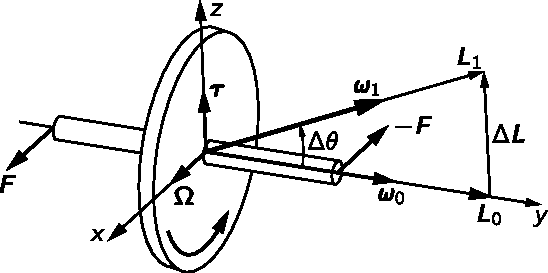
\includegraphics[width=0.9\linewidth]{fyz_fig407.pdf}
      \caption{Setrvačník
               (\cite[s.~279]{Feynman01})}
      \label{fyz:fig407}
    \end{figure}

    Mají-li oba vektory \(\vec{\Omega}\) a \(\vec{L}_0\) horizontální směr, jako je to na obrázku,
    potom \(\vec{N}\) má \emph{vertikální} směr. K vytvoření takového momentu síly jsou potřebné
    síly \(\vec{F}\) a \(-\vec{F}\) na obou koncích osy kola. Odkud pocházejí tyto síly? Způsobíme
    je našima rukama při změně polohy rotační osy kola. Podle třetího Newtonova zákona stejně velké,
    ale opačné síly (stejně velké, ale opačné \emph{momenty}) působí na \emph{nás}. To způsobí, že
    se začneme otáčet v opačném směru kolem osy \(z\).   
    
    \begin{figure}[ht!] %\ref{fyz:fig408}
      \centering
      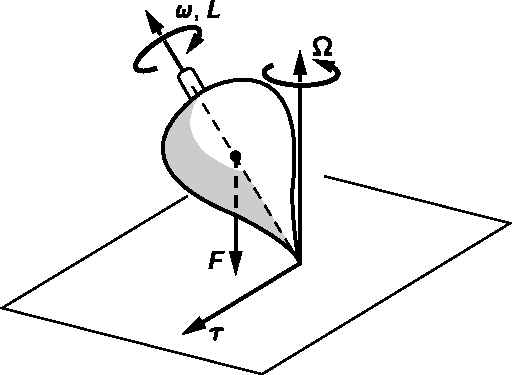
\includegraphics[width=0.9\linewidth]{fyz_fig408.pdf}
      \caption{Rychle se otáčející káča. Směr vektoru momentu síly je směrem precese 
               (\cite[s.~280]{Feynman01})}
      \label{fyz:fig408}
    \end{figure}

    Poslední poznatek lze zobecnit i na rychle se otáčející „dětskou káču“. V tomto známém případě
    vlastní tíha působící v těžišti vytváří moment síly vzhledem k bodu dotyku s podlahou (obr.
    \ref{fyz:fig408}). Tento moment síly má horizontální směr a způsobuje precesní pohyb rotační osy
    káčy po plášti rotačního kužele kolem svislé přímky. Je-li (vertikální) úhlová rychlost precese
    \(\vec{\Omega}\) máme znovu
    \begin{equation*}
      \vect{N} = \der{\vec{L}}{t} = \vec{Ω} \times \vec{L}_0.
    \end{equation*}

    Takže působíme-li na rychle se otáčející káču momentem síly, je směr precesního pohybu ve směru
    momentu síly, tedy, pod pravými úhly vzhledem k silám způsobujícím daný moment síly.

    Nyní můžeme tvrdit, že chápeme precesní pohyb setrvačníků. Ve skutečnosti ho chápeme po
    matematické stránce. V určitém smyslu se celá věc jeví jako \uv{zázrak}. Když budeme probírat
    složitější fyziku, ukáže se, že mnohé jednoduché jevy lze odvodit matematicky mnohem rychleji,
    než je lze skutečně pochopit. Je to podivuhodné a jakmile přejdeme ke složitějším problémům,
    uvidíme, že matematicky dostaneme výsledky, jímž v podstatě nikdo nebyl schopen přímo porozumět.
    Příkladem je \emph{Diracova rovnice}, jež má velmi pěkný a jednoduchý tvar, ale jejíž důsledky
    lze těžko pochopit. V našem případě se jeví precesní pohyb jako nějaký zázrak sestávající z
    pravých úhlů, kruhů, pootočení a pravotočivých šroubů. Měli bychom se pokusit pochopit hlubší
    fyzikální smysl věci.
    
    Jak lze vysvětlit moment síly pomocí skutečných sil a zrychlení? Všimněme si, že když rotující
    těleso vykonává precesní pohyb, nerotují částice kola ve skutečnosti v rovině (obr.
    \ref{fyz:fig409}). Jak jsme si dříve vysvětlili (obr. \ref{fyz:fig405}), částice, které právě
    nyní procházejí osou precesního pohybu, se pohybují po \emph{zakřivených trajektoriích}, a to
    znamená, že na ně působí síla ze strany. Ta je vytvořena naším tlakem na osu, a přenáší se
    špicemi až na rám kola. „Počkat“, někdo řekne, „ale co s částicemi, jež se pohybují opačně na
    druhé straně?“ Rychle lze rozhodnout, že na druhé straně musí působit \emph{opačná síla}.
    Výsledná síla, jíž musíme působit, je proto rovna nule. Síly jsou vyvážené, ale jedna z nich
    musí působit na jednom konci kola a druhá na druhém. Těmito silami bychom mohli působit přímo,
    ale protože kolo je tuhé, stačí působit najeho osu a síly se přenesou dále na obvod.

    \begin{figure}[ht!] %\ref{fyz:fig409}
      \centering
      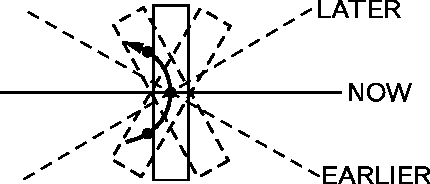
\includegraphics[width=0.9\linewidth]{fyz_fig409.pdf}
      \caption{Při otáčení osy vykonávají částice rotujícího kola (obr. \ref{fyz:fig407}) pohyb, 
               který se děje po zakřivených trajektoriích 
               (\cite[s.~280]{Feynman01})}
      \label{fyz:fig409}
    \end{figure}

    Zatím jsme dokázali, že pomocí precesního pohybu může kolo vyvážit moment síly způsobený
    gravitací nebo jiný moment síly, jenž na něj působí. Přitom všechno, co jsme dokázali je, že
    takovýto pohyb je jedním řešením nějaké rovnice. Je-li tedy dán moment síly a máme-li těleso,
    které\emph{nerušeně rotovalo}, pak bude vykonávat precesní pohyb hladce a rovnoměrně. Ale
    nedokázali jsme (a ani to není pravda), že rovnoměmá, regulární precese je \emph{nejobecnějším}
    pohybem, jejž může vykonávat rotující těleso pod vlivem daného momentu síly. Obecný pohyb
    zahrnuje i oscilace kolem středního precesního pohybu, jimž se říká \textbf{nutace}.

    \begin{figure}[ht!] %\ref{fyz:fig410}
      \centering
      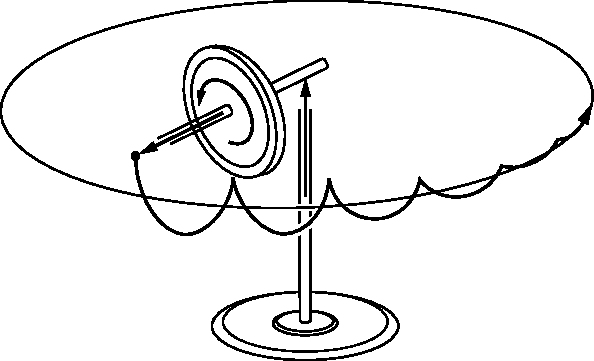
\includegraphics[width=0.9\linewidth]{fyz_fig410.pdf}
      \caption{Skutečný pohyb konce setrvačníku pod vlivem tíhy ihned po uvolnění předtím uchycené
               osy (\cite[s.~281]{Feynman01})}
      \label{fyz:fig410}
    \end{figure}

    Někteří lidé rádi říkají, že když na setrvačník působí moment síly, začne vykonávat precesní
    pohyb, a že moment síly \emph{způsobuje} precesi. Velmi zvláštní je to, že když uvolníme
    setrvačník, pak pod vlivem tíhy nespadne, ale místo toho se začne pohybovat do strany! Jak to,
    že svislá tíhová síla, která směřuje dolů a kterou známe a cítíme, způsobí, že se setrvačník
    bude pohybovat do strany? Všechny vzorce světa jako je (\ref{fyz:eq724}) nám to neřeknou, neboť
    (\ref{fyz:eq724}) je speciální rovnice a platí jen pro regulární precesní pohyb setrvačníku. Co
    se ve skutečnosti dopodrobna odehraje, je toto. Kdybychom rotační osu drželi zcela pevně, takže
    by precesní pohyb vůbec nemohl nastat (ale setrvačník by rotoval), nepůsobil by žádný moment
    síly, dokonce ani moment síly způsobený tíhou, neboť bychom ho vyvažovali svými prsty. Kdybychom
    ale náhle setrvačník pustili, okamžitě by se uplatnil tíhový moment síly. Každý, kdo má zdravý
    rozum, by si myslel, že setrvačník začne padat, a to skutečně začne, což lze vidět, nerotuje-li
    příliš rychle.

    Setrvačník skutečně padá, jak bychom očekávali. Ale jen co začne padat, začne se otáčet, a k
    tomu, aby tento otáčivý pohyb pokračoval, je třeba momentu síly. Za nepřítomnosti momentu síly v
    tomto směru, začne setrvačník „padat“ v opačném směru, tj. ve směru chybějící síly, jež měla
    horizontální směr. To způsobí pohyb setrvačníku kolem vertikální osy, jaký by měl při regulární
    precesi. Skutečný pohyb přitom překročí rychlost regulámí precese a rotační osa se zvedne na
    úroveň, z níž začala padat. Trajektorie opisovaná volným koncem osy, je \emph{cykloida} (takovou
    trajektorii opisuje například kamínek zachycený v rýze na pneumatice auta). Tento pohyb je
    obvykle příliš rychlý na to, abychom ho mohli postřehnout, rychle se utlumí v důsledku tření
    vložiskách závěsu a zůstane jen regulární precesní pohyb (obr. \ref{fyz:fig410}). Čím pomaleji
    kolo rotuje, tím je nutace zřetelnější.

    Když se pohyb ustálí, osa setrvačníku je o něco níže než na začátku. Proč? To jsou složitější
    detaily, ale zmiňujeme se o nich, protože nechceme, aby čtenář měl dojem, že setrvačník je
    absolutní zázrak. Je to nádherná věc, ale není to žádný zázrak. Kdybychom osu drželi zcela
    vodorovně a najednou ji pustili, pak zjednoduché rovnice precese zjistíme, že se bude otáčet ve
    vodorovné rovině. Ale to je nemožné! Ačkoli jsme to předtím zanedbali, je pravda, že kolo má
    určitý moment setrvačnosti kolem precesní osy a pohybuje-li se kolem této osy, i když jen
    pomalu, má malý moment hybnosti vzhledem k této ose. Odkud se vzal? Jsou-li čepy dokonalé, pak
    není žádný moment síly vzhledem k vertikální ose. Jak to, že začne precesní pohyb, jestliže se
    nezměnil moment hybnosti? Odpověď je následující: Cykloidální pohyb konce osy se utlumí na
    rovnoměmý pohyb středu myšlené valící se kružnice. To znamená, že se ustálí trochu níže. Protože
    je níže, rotační moment hybnosti má malou vertikální složku, což je přesně to, co je třeba k
    precesnímu pohybu. Takže rotační osa musela trochu klesnout, aby se mohla začít pohybovat
    dokola. Musela se trochu poddat gravitaci; tím, že se trochu sklonila, zachovala si rotaci kolem
    vertikální osy. Tak se tedy pohybuje setrvačník.

  \section{Moment hybnosti tuhého tělesa}\label{fyz:IchapXXsecIV}
    Dříve, než zanecháme trojrozměrné rotace, podívejme se, alespoň kvalitativně, na několik jevů,
    jež nejsou zcela samozřejmé, a jež se vyskytují při trojrozměrných rotacích. Nejvýraznější
    zvláštností je to, že obecně moment hybnosti tuhého tělesa \emph{nemá nutně} stejný směr, jako
    úhlová rychlost. Podívejme se na kolo, které je upevněno šikmo na ose, jež prochází jeho
    těžištěm (obr. \ref{fyz:fig411}). Když roztočíme takové kolo kolem osy, každý ví, že se budou
    chvět ložiska, neboť kolo jsme upevnili šikmo. Kvalitativně víme, že v rotujícím systému působí
    na kolo odstředivá síla, která se snaží odhodit hmotu kola co nejdál od osy otáčení. Tato síla
    má tendenci vyrovnat rovinu kola, aby byla kolmá na osu. K překonání této tendence působí
    ložiska momentem síly. Působí-li ložiska momentem síly, musí docházet k změně momentu hybnosti.
    Jak se může při prostém otáčení kola kolem osy měnit moment hybnosti? Předpokládejme, že
    rozložíme úhlovou rychlost \(\vec{\Omega}\) na složky \(\vec{\Omega}_1\) a \(\vec{\Omega}_2\),
    kolmou a podélnou složku s rovinou kola. Čemu je roven moment hybnosti?

    \begin{figure}[ht!] %\ref{fyz:fig411}
      \centering
      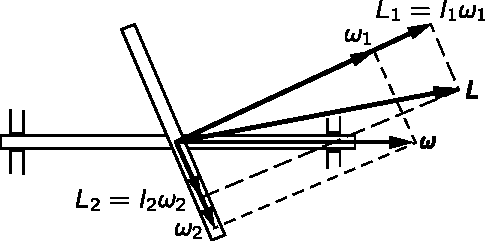
\includegraphics[width=0.9\linewidth]{fyz_fig411.pdf}
      \caption{Moment hybnosti rotujícího tělesa není nutně rovnoběný s úhlovou rychlostí
              (\cite[s.~282]{Feynman01})}
      \label{fyz:fig411}
    \end{figure}

    Momenty setrvačnosti vzhledem k těmto osám jsou rozdílné, takže složky momentu hybnosti, jež
    jsou rovny součinům momentů setrvačnosti a příslušné složky úhlové rychlosti, jsou (jen pro
    takto speciálně zvolené osy) v jiném poměru než složky úhlové rychlosti. Vektor momentu hybnosti
    tedy nemíří ve směru osy otáčení kola. Otáčíme-li kolo, otáčíme v prostoru i vektor momentu
    hybnosti, takže na osu musíme působit momentem síly.

    Ačkoli je to příliš komplikované na dokazování, moment setrvačnosti má velmi důležitou a
    zajímavou vlastnost, kterou lze snadno popsat a používat, a která tvoří základ naší
    předcházející analýzy. Je to tato vlastnost: Každé tuhé těleso, dokonce i tak nepravidelné jako
    brambora, má tři navzájem kolmé osy procházející těžištěm, takové, že moment setrvačnosti
    vzhledem k jedné z nich má \emph{největší možnou} hodnotu z hodnot určených vůči libovolným osám
    procházejícím těžištěm. Moment setrvačnosti vzhledem k další z nich má \emph{nejmenší možnou}
    hodnotu a moment setrvačnosti vzhledem k třetí ose má velikost mezi prvními dvěma (nebo je roven
    některé z nich). Tyto osy se nazývají \textbf{hlavními osami} tělesa a mají tu zvláštní
    vlastnost, že když se těleso otáčí kolem některé z nich, má moment hybnosti stejný směrjako
    úhlová rychlost. V tělese, které má osy symetrie, míří hlavní osy podél os symetrie.

    \begin{figure}[ht!] %\ref{fyz:fig412}
      \centering
      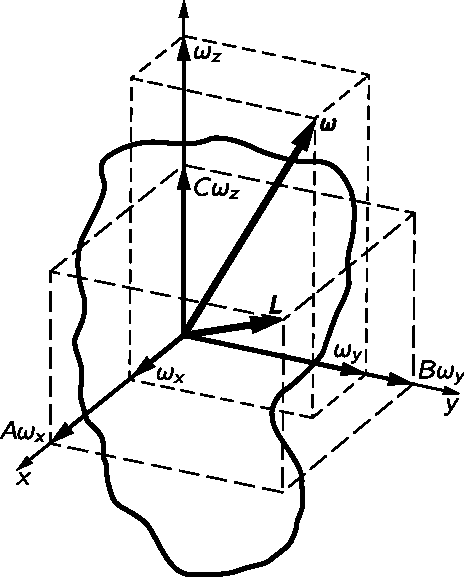
\includegraphics[width=0.9\linewidth]{fyz_fig412.pdf}
      \caption{Úhlová rychlost a moment hybnosti tuhého tělesa (\(A>B>C\))
              (\cite[s.~283]{Feynman01})}
      \label{fyz:fig412}
    \end{figure}

    Ztotožníme-li souřadnicové osy \(x\), \(y\), \(z\) s hlavními osami a odpovídající hlavní
    momenty setrvačnosti nazveme \(A\), \(B\) a \(C\), můžeme snadno vypočítat moment hybnosti a
    kinetickou energii rotujícího tělesa pro jakoukoli úhlovou rychlost \(\omega\).

    Rozložíme-li \(\vec{\omega}\) na složky \(ω_x\), \(ω_y\) a \(ω_z\) podél os \(x\), \(y\) a
    \(z\), můžeme psát moment hybností s použitím jednotkových vektorů \(\vec{i}\), \(\vec{j}\),
    \(\vec{k}\), směřujících podél \(x\), \(y\) a \(z\) jako 
    \begin{equation}\label{fyz:eq725}
      \vec{L}=Aω_x\vec{i}+Bω_y\vec{j}+Cω_z\vec{k}.
    \end{equation}
    Kinetická energie rotace je
    \begin{equation}\label{fyz:eq726}
      E_k=\frac{1}{2}(Aω^2_x+Bω^2_y+Cω^2_z) =\frac{1}{2}\vec{L}\cdot\vec{ω}. 
    \end{equation}

  \section{Příklady a cvičení}\label{fyz:IchapXXsecV}  

%---------------------------------------------------------------------------------------------------